\subsubsection{Angular}

\begin{flushleft}
  \textbf{Správa stavů, předávání vlastností}
\end{flushleft}

Pro implementaci jednoduchého counteru nejprve vytvoříme counter komponentu. Můžeme začít se strukturou HTML značek pro hlavní komponentu.

\begin{prog}
// Soubor counter.component.html

<div class="bg-gray-200 p-6 rounded-md shadow-md">
  <p class="text-xl font-semibold mb-4">Current count: \{\{ count \}\}</p>

  <div class="flex gap-4">
    <counter-button
      [className]="'bg-blue-500 text-white hover:bg-blue-600'"
      (buttonClicked)="increment()"
    >
      Increment
    </counter-button>

    <!-- další tlačítka... -->
  </div>
</div>
\end{prog}

Jelikož potřebujeme opakovaně použít logiku jednotlivých tlačítek, vytvoříme komponentu counter-button. 
Ta může přijímat například CSS styly nebo přes output (\emph{EventEmitter}) posílat informaci o~kliknutí na tlačítko směrem nahoru ve stromě komponent.

\begin{prog}
// Soubor counter-button.component.ts

import \{CommonModule\} from '@angular/common';
import \{Component, EventEmitter, Input, Output\} from '@angular/core';

// Nastavení komponenty.
@Component(\{
  selector: 'counter-button',
  standalone: true,
  templateUrl: './counter-button.component.html',
  imports: [CommonModule],
\})
export class CounterButtonComponent \{
  // Vstupní vlastnost komponenty.
  @Input() public className = '';

  // Výstupní vlastnost komponenty.
  @Output() public buttonClicked = new EventEmitter<void>();
\}
\end{prog}

Funkci \emph{emit()} \emph{EventEmitteru} zavoláme na tlačítku v~counter-buttonu právě tehdy, když uživatel klikne na tlačítko -- použijeme listener ve formě \emph{(click)}. 
K~propsání textu či jiných elementů nebo komponent mezi párovými tagy <counter-button> pak poslouží párový či nepárový element <ng-content />.

\begin{prog}
// Soubor counter-button.component.html

<button
  class="px-4 py-2 rounded-md focus:outline-none"
  [ngClass]="className"
  (click)="buttonClicked.emit()"
>
  <!-- ng-content slouží k vykreslení obsahu, který vložíme
    mezi párové tagy (selectory) dané komponenty. -->
  <ng-content></ng-content>
</button>
\end{prog}

Následně v~counter komponentě importujeme třídu CounterButtonComponent a~do všech elementů counter-button předáme jejich vstupy a~výstupy. 
Námi definovanovanému outputu \emph{buttonClicked} předáme v~šabloně metodu, která se vykoná po emitu (kliknutí na tlačítko ve vnořené komponentě) a~metodu zavoláme pomocí kulatých závorek. 
V~rámci counter komponenty pak definujeme stav jako vlastnost \emph{count} na třídě. Vlastnost pak můžeme modifikovat skrze metody třídy, které voláme v~outputu \emph{buttonClicked}.

\begin{prog}
// Soubor counter.component.ts

import \{CommonModule\} from '@angular/common';
import \{Component\} from '@angular/core';
import \{CounterButtonComponent\} from './button/counter-button.component';

@Component(\{
  selector: 'counter',
  standalone: true,
  templateUrl: './counter.component.html',
  imports: [CommonModule, CounterButtonComponent],
\})
export class CounterComponent \{
  protected count = 0;

  protected increment(): void \{
    this.count++;
  \}

  protected decrement(): void \{
    this.count--;
  \}

  protected reset(): void \{
    this.count = 0;
  \}
\}
\end{prog}

\begin{flushleft}
  \textbf{Interakce v uživatelském prostředí}
\end{flushleft}

Při vytváření jakékoli UI komponenty můžeme začít šablonou, nebo definovat funkční stránku. My začneme s~tvorbou šablony. V~případě vlastního dropdown samotným tlačítkem a~seznamem možností. 
Otevření možností zajístíme tak, že na tlačítko přidáme click listener. Funkčnost pak zajistíme díky modifikaci stavu \emph{isOpen}, který se provede při volání metody \emph{toggleDropdown}. 
V~rámci této metody je třeba zavolat i~\emph{event.stopPropagation()}. Předejdeme tak potenciální chybě ve formě tzv. event bubblingu -- spuštění událostí na prvcích odlišných od cílového.

\begin{prog}
// Část souboru dropdown.component.html

<div class="rounded-md shadow-sm">
  <!-- Pro poslouchání na události v DOMu můžeme 
    použít syntaxi: (NÁZEV_UDÁLOSTI)="OBSLUŽNÁ_METODA". -->
  <button
    type="button"
    class="" <!-- Statické styly... -->
    [ngClass]="buttonStyles + ' ' + sizeStyles"
    (click)="toggleDropdown(\$event)"
  >
    \{\{ selectedOption ? selectedOption.label : placeholder \}\}
    <!-- Pro podmíněné vykreslovaní můžeme využít bloky @if, @else if, @else. -->
    @if (isOpen) \{
      <arrow-up-icon />
    \} @else \{
      <arrow-down-icon />
    \}
  </button>
</div>
\end{prog}

Podmíněně zobrazíme seznam možností, které získáme v~jednom z~inputů. K~vykreslení všech možností použijeme blok \emph{@for}. 
Pro vybraní konkrétní možnosti využijeme \emph{(click)} a~do obslužné metody předáme aktuální prvek v~poli -- option. 
Metoda \emph{handleOptionClick} pak zajistí uložení aktuálně vybrané možnosti, zavření dropdownu a~vyemitování vybrané možnosti do rodičovské komponenty.

\begin{prog}
// Část souboru dropdown.component.html

@if (isOpen) {
  <div
    class="" <!-- Statické styly... -->
    [ngClass]="divStyles"
  >
    <div class="py-1" role="menu"> <!-- WAI-ARIA atributy... -->
      <!-- Pro vykreslení listu (pole hodnot) můžeme využít blok @for. -->
      @for (option of options; track option.value) {
        <button
          class="block w-full text-left px-4 py-2 text-sm hover:text-gray-900"
          [ngClass]="optionStyles"
          role="menuitem"
          (click)="handleOptionClick(option)"
        >
          {{ option.label }}
        </button>
      }
    </div>
  </div>
}
\end{prog}

V~případě, že máme dropdown otevřen a~chceme jej po kliknutí mimo tentýž dropdown bezpečně zavřít, nehledě na počet vykreslených dropdown komponent na stránce, budeme postupovat následovně. 
Pro každou komponentu vytvoříme unikátní vlastnost ve formě ID. To pak dynamicky umístíme na kořenový element dropdownu.

\begin{prog}
// Část souboru dropdown.component.ts

protected dropdownId = `id-\${crypto.randomUUID()}`;

// Část souboru dropdown.component.html

<div class="relative inline-block text-left" [id]="dropdownId">
\end{prog}

V~komponentě pak budeme naslouchat na události v~DOM pomocí dekorátoru \emph{@HostListener}. 
Dekorátor přijímá DOM událost, na který má poslouchat -- \emph{document:pointerdown}, případně další argumenty nebo také formu vypublikované události. 
Pod dekorátorem pak definujeme obslužnou metodu, která se volá při emitu specifikované události. V~rámci metody pak zajistíme uzavření aktuálně otevřeného dropdownu.

\begin{prog}
// Část souboru dropdown.component.ts

@HostListener('document:pointerdown', ['\$event.target'])
onClickOutsideDropdown(target: HTMLElement): void \{
  if (this.isOpen && !target.closest(`#\$\{this.dropdownId\}`)) \{
    this.isOpen = false;
  \}
\}
\end{prog}

Dropdown pak může mít různé inputy, které povedou k~lepší znovupoužitelnosti. Hodnotu inputu (konkrétně např.~\emph{defaultValue}) v~komponentě získáme v~metodě životního cyklu \emph{OnInit}. 
Styly ve formě JS hodnot do šablony přidáme pomocí \emph{ngClass}. Když těchto hodnot potřebujeme na elementu více, zřetězíme předávané hodnoty pomocí JavaScriptu. 
Další možnost spočívá ve sloučení požadovaných stylů na úrovni třídy.

\begin{flushleft}
  \textbf{Reaktivita, asynchronní operace}
\end{flushleft}

Pro ukázku reaktivity a~asynchronních operací můžeme vytvořit komponentu, která bude překládat zadaný text do vybraného jazyka. 
Začneme tedy vytvořením rodičovské komponenty, která při změně vlastností (zadaného textu uživatelem a~výstupního jazyka) zavolá API, které vrátí přeložený text. 
V~rámci této komponenty vytvoříme vnořené komponenty, které budou sloužit k~zadání vstupního textu, výběru jazyka a~zobrazení výsledku. 

LanguageDropdownComponent umožní uživateli vybrat jazyk, do kterého chce přeložit text. 
Přes \emph{EventEmitter} aktualizujeme výstupní jazyk v~rodičovské komponentě. V~rámci obslužné metody \emph{handleLanguageChange} pak také modifikujeme hodnotu vlastnosti \emph{inputValuesChanges\$}.
Tato vlastnost je \emph{Subject}, speciální typ observable, z~knihovny RxJS. Později dovolí na základě změny hodnoty poslat dotaz na server ve správný moment. 
Podobným způsobem poté můžeme registrovat událost změny vstupního textu -- naslouchat na změnu vstupního textu.
% TODO: Přidat schéma

\begin{prog}
// Část souboru translator.component.ts

protected handleLanguageChange(outputLanguage: Option): void \{
  this.outputLanguage = outputLanguage.value;
  // Synchronní aktualizace hodnoty observable (v tomto případě Subjectu).
  // Slouží pro následné operace při změně hodnoty observable.
  this.inputValuesChanges\$.next(outputLanguage.value);
\}
\end{prog}

Zadání vstupního textu pak může řešit komponenta TranslationInputComponent, která obdobným způsobem aktualizuje hodnotu vstupního textu v~rodičovské komponentě. 
Aktuální hodnotu formulářového prvku nastavíme pomocí \emph{[ngModel]}. Pro naslouchání na změnu hodnoty formulářového prvku zase využijeme \emph{(ngModelChange)}.

\begin{prog}
// Část souboru translation-input.component.html

<textarea
  autosizeTextArea
  class="block w-full min-h-0 p-3 pr-12 pb-8 resize-none !outline-none"
  placeholder="Type to translate ..."
  [ngModel]="inputText"
  (ngModelChange)="handleInputChange(\$event)"
>
</textarea>
\end{prog}

V~případě, že potřebujeme aktualizovat výšku textového pole na základě jeho obsahu, můžeme využít vlastní direktivu AutosizeTextAreaDirective. 
V~konstruktoru direktivy získáme element, na který přidáme tuto direktivu. Dále budeme potřebovat třídu \emph{Renderer2}, která umožňuje manipulovat s~DOM. 
V~direktivě budeme naslouchat na změnu hodnoty textového pole pomocí dekorátoru \emph{@HostListener} a~události input. Následně v~rámci obslužné metody zajistíme aktualizaci výšky.

Změny hodnoty vlastnosti \emph{inputValuesChanges\$} začneme odebírat pomocí \emph{subscribe}. 
Abychom předešli dotazování serveru ihned po změně hodnoty vlastnosti \emph{inputValuesChanges\$}, použijeme operátor \emph{debounceTime}. 
Ten povolí poslat dotaz na server až po uplynutí určité doby od poslední změny, kterou můžeme nastavit. 
Subscribe zavolá veřejnou metodu služby (\emph{getTranslation}), která vrací přeložený text. 
Nakonec, aby dotazování serveru fungovalo, je třeba metodu \emph{setupInputChangeSubscription} zavolat v~konstruktoru nebo hooku \emph{OnInit}.

\begin{prog}
// Část souboru translator.component.ts

private setupInputChangeSubscription(): void \{
  // Naslouchá změnám vstupního textu a výstupního jazyka.
  // Operátor debounceTime zajistí, že se změna vstupního textu 
    nebo výstupního jazyka vyhodnotí až po uplynutí 300 ms.
  // Dále operátor distinctUntilChanged zajišťuje, 
    že se změna vyhodnotí pouze v případě, kdy je odlišná od předchozí hodnoty.
  // Operátor takeUntil() zajišťuje, 
    že se subscription zruší při zničení komponenty.
  // Pokud se změní vstupní text nebo výstupní jazyk, 
    v rámci methody subscribe se spustí překlad.
  this.inputValuesChanges\$
    .pipe(debounceTime(300), distinctUntilChanged(), takeUntil(this.destroy\$))
    .subscribe(() => this.triggerTranslation());
\}
\end{prog}

V~rámci služby TranslationService použijeme třídu \emph{HttpClient} z~Angular modulů, která umožňuje odesílat HTTP požadavky na server.
Službu \emph{HttpClient} získáme v~konstruktoru, kde ji pomocí klíčového slova \emph{private} přiřadíme do vlastností třídy. 
Pokračujeme implementací metody \emph{getTranslation}, v~níž zavoláme metodu \emph{post} na HTTP klientovi s~patřičným nastavením. 
Tímto způsobem budeme dotazovat Microsoft Translator Text API \cite{translatortextapi}, díky kterému v~odpovědi obdržíme přeložený text. 
Pokud úspěšná odpověď ze serveru obsahuje složitější strukturu, ze které potřebujeme získat jen nějakou část, pak s~konverzí odpovědi pomůže RxJS operátor \emph{map()}. 
Metoda \emph{getTranslation} vrací observable, v~translator komponentě proto hodnoty odebíráme pomocí metody \emph{subscribe}. 
Subscription bychom také vždy měli zrušit, abychom předešli možným únikům paměti či chybám.

\begin{prog}
// Část souboru translation.service.ts

return this.httpClient
  .post<TranslationResponseData>(url, body, options)
  .pipe(map(data => this.convertToOutputText(data)));

// Část souboru translator.component.ts

// Slouží ke zrušení subscriptions při zničení komponenty.
private destroy\$: Subject<void> = new Subject();
// Slouží k naslouchání na změny vstupního textu a výstupního jazyka.
private inputValuesChanges\$ = new Subject<string>();

public ngOnDestroy(): void \{
  // Slouží k manuálnímu unsubscribe všech observables při zničení komponenty.
  this.destroy\$.next();
  this.destroy\$.complete();
\}

this.translationService
  .getTranslation(this.inputText, this.outputLanguage)
  .pipe(
    // Zajišťuje, že se subscription zruší při zničení komponenty.
    takeUntil(this.destroy\$),
    // Zachytí chybu v observable.
    catchError(error => this.handleError(error)),
  )
  // V metodě subscribe dostaneme transformovanou odpověď 
    (v rámci next callbacku) nebo chybu (v rámci error callbacku).
  // Po poslední úspěšné aktualizaci observable se volá callback funkce complete.
  .subscribe(\{
    next: response => (this.outputText = response),
    error: error => (this.error = error),
    complete: () => (this.loading = false),
  \});
\end{prog}

V~momentě, kdy obdržíme odpověď ze serveru, zobrazíme přeložený text uživateli. 
K~tomu poslouží TranslationOutputComponent, které na vstupu předáme výstupní text spolu s~dalšími vstupními vlastnostmi. 
V~rámci šablony pak podmíněně vykreslíme přeložený text, chybu nebo načítání. 

Při zarovnání vstupního a~výstupního pole v~UI si musíme dát pozor na to, že šířku je potřeba nastavit již v~prvním potomku div elementu, na kterém nastavíme flexbox. 
Důvod spočívá v~tom, že Angular v~DOM vytváří element pro každou komponentu.

\begin{prog}
// Část souboru translation.service.ts

<div class="flex text-xl">
  <translation-input 
    <!-- Vstupní a výstupní vlastnosti... -->
    class="relative w-1/2"
    <!-- Šířka musí být nastavena zde. -->
  />

  <translation-output 
    <!-- Vstupní a výstupní vlastnosti... -->
    class="relative w-1/2"
    <!-- Šířka musí být nastavena zde. -->
  />
</div>
\end{prog}

\begin{flushleft}
  \textbf{Tvorba formulářů, validace}
\end{flushleft}

Angular je flexibilní z~pohledu možností tvorby formulářů. My použijeme reaktivní formuláře, jelikož jsou flexibilnější a~umožní nám jednodušší reakce na změny prvků.
Vytvoříme komponentu zaměřenou na jednoduché investiční kalkulace. 
Bude obsahovat dvě vnořené komponenty: formulář pro zadání vstupních dat a~komponentu výsledku kalkulace, která se zobrazí po potvrzení formuláře.

Začneme s~tvorbou reaktivního formuláře. Typ \emph{InvestForm} popisuje strukturu souvisejících formulářových prvků formuláře.

\begin{prog}
// Část souboru invest-form.component.ts

type InvestForm = FormGroup<\{
  oneOffInvestment: FormControl<number | null>;
  investmentLength: FormControl<number | null>;
  averageSavingsInterest: FormControl<number | null>;
  averageSP500Interest: FormControl<number | null>;
\}>;
\end{prog}

Protože prvků budeme mít více, deklarujeme formulářovou skupinu jako vlastnost třídy, ve které následně definujeme samotné formulářové prvky. 
Vlastnost \emph{investForm} pak umožní přístup k~hodnotám formuláře a~jeho validaci. Zde narazíme na problém s~nenastavením počáteční hodnoty vlastnosti přímo nebo v~konstruktoru. 
Můžeme ho vyřešit za pomoci vykřičníku -- řekneme tak TypeScriptu, že obsah proměnné je nenulový. Další možností je vypnout pravidlo \emph{strictPropertyInitialization} v~souboru \emph{tsconfig.json}.

\begin{prog}
// Část souboru invest-form.component.ts

protected investForm!: InvestForm;
\end{prog}

Hodnotu vlastnosti \emph{investForm} nastavíme pomocí metody \emph{initializeInvestForm} v~rámci \emph{OnInit} hooku. 
Tento postup zvolíme, protože chceme nastavovat počáteční hodnoty formuláře na základě vstupní vlastnosti \emph{defaultValues}.
Důvodem je, že hodnoty vstupních vlastností jsou v~komponentě dostupné nejdříve v~rámci hooku \emph{OnInit}.

Metoda \emph{initializeInvestForm} vrátí instanci třídy \emph{FormGroup}, kterou vytvoříme pomocí třídy \emph{FormBuilder} ze základního balíčku \emph{@angular/forms}. 
Argumentem pro metodu \emph{group} pak je objekt, který popisuje strukturu formuláře. 
Vlastnosti objektu budou klíče formulářových prvků a~jejich hodnoty pole, kde první prvek bude počáteční hodnota a~druhý prvek pole validátorů.

\begin{prog}
// Část souboru invest-form.component.ts

private initializeInvestForm(): InvestForm \{
  // Vytvoření formuláře s výchozími hodnotami 
    (případně vlastnostmi) a validátory.
  // Jednotlivé prvky FormGroup bývají označovány jako FormControl.
  return this.fb.group(\{
    oneOffInvestment: [
      this.defaultValues.oneOffInvestment,
      [Validators.required, Validators.min(20), Validators.max(99_999_999)],
    ],
    // Další formulářové prvky... 
  \});
\}
\end{prog}

V~šabloně následně propojíme formulářovou skupinu s~formulářem. K~tomu poslouží direktiva \emph{[formGroup]} a~její hodnotu nastavíme na vlastnost \emph{investForm}. 
V~rámci formuláře pak vytvoříme formulářové prvky, které propojíme direktivou \emph{formControlName}. Hodnota pak musí odpovídat klíči prvku ve formulářové skupině. 
Pro zajištění efektivní obsluhy chyb formuláře můžeme využít getter metody, které vrátí konkrétní formulářový prvek.

\begin{prog}
// Část souboru invest-form.component.html

<form [formGroup]="investForm" (ngSubmit)="onSubmit()">
  <div class="md:flex md:gap-4">
    <div class="mb-4 md:w-1/2">
      <input-label id="oneOffInvestment">
        One-off investment (20-99.999.999€)
      </input-label>

      <!-- Direktiva formControlName slouží k propojení inputu 
        s odpovídajícím FormControl v FormGroup. -->
      <input
        id="oneOffInvestment"
        type="number"
        formControlName="oneOffInvestment"
        class="" <!-- Statické styly... -->
      />

      @if (oneOffInvestmentControl.errors?.['required']) \{
        <p class="text-red-500 text-xs italic mt-1">
          Please enter a valid amount of one-off investment (positive number).
        </p>
      \}
      <!-- Další chybové hlášky... -->
    </div>

    <!-- Další formulářové prvky... -->
  </div>
</form>
\end{prog}

Dále vytvoříme tlačítko s~typem submit, přes které uživatel formulář potvrdí. Na form značku přidáme \emph{(ngSubmit)}, který vyemituje událost při potvrzení formuláře. 
Obslužná metoda pak prostřednictvím výstupové vlastnosti publikuje aktuální hodnotu reaktivního formuláře do rodičovské komponenty.

V~rámci rodičovské komponenty tedy vykreslíme samotný formulář a~při jakémkoli potvrzení formuláře získáme aktuální hodnoty z~formuláře díky outputu. 
Hodnoty formuláře pak dostaneme v~obslužné metodě \emph{handleFormChanged}. Pomocí služby FutureValuesCalculatorService tyto hodnoty transformujeme do požadovaného formátu. 
Výsledek uložíme do vlastnosti \emph{futureValues}.

Když jsou hodnoty vypočteny, vykreslíme je na stránce prostřednictvím komponent future-values-info a~future-value-info. 
První z~komponent slouží k~rozložení výsledků do požadovaného formátu a~vytvoření komponent pro jednotlivé výsledky. 
Komponenta future-value-info pak přijímá vstupní vlastnost, kterou v~šabloně před vykreslením v~DOM přetransformujeme díky rouře (\emph{LocalizedNumberPipe}).

\begin{prog}
// Část souboru future-value-info.component.html

<p class="text-5xl font-bold">{{ futureValue | localizedNumber }}</p>
\end{prog}

Stejného výsledku bychom mohli dosáhnout i~přes metodu na třídě. Tento přístup Angular nedoporučuje, jelikož metody se v~rámci šablony spouští opakovaně a~mohou způsobit problémy s~výkonem. 
Oproti tomu roura umožní lepší znovupoužitelnost a~přehlednost.

\begin{prog}
// Soubor localized-number.pipe.ts

import {Pipe, PipeTransform} from '@angular/core';

// Roura, která převede číslo na formátovaný string s měnou (€).
@Pipe(\{name: 'localizedNumber', standalone: true\})
export class LocalizedNumberPipe implements PipeTransform \{
  public transform(value: number): string \{
    return `\$\{value.toLocaleString('de-DE')\}€`;
  \}
\}
\end{prog}

\begin{flushleft}
  \textbf{Modularita, použití knihoven}
\end{flushleft}

V~této sekci vytvoříme webovou hru, kde cílem uživatele bude uhádnout název státu na základě poskytnutých nápověd. Práci si ulehčíme pomocí externích knihoven a~služeb.
Ve hře se postupně bude odkrývat 8 nápověd, které by měly pomoct s~uhádnutím daného státu. 
Klíčovým prvkem je textové pole, přes které uživatel zadává názvy hádaných zemí a~tlačítko pro potvrzení. 
Součástí je také seznam již zadaných hádaných zemí a~modální okna sloužící k~vyhodnocení hry.

Začneme s~implementací rodičovské komponenty, která bude získávat data o~všech zemích světa z~REST Countries API\footnote{REST Countries API je dostupné pod Mozilla Public License~2.0.\cite{restcountriesapi}}. 
Další zodpovědností této komponenty bude vykreslování odpovídajících stavů při získávání dat -- stav načítání, úspěšné získání dat a~chyba při získávání dat. 
Vytvoříme službu CountryService, díky které získáme data o~zemích. Pro tyto účely vytvoříme metodu \emph{getAllCountries}, která vrátí observable pole všech zemí. 
Výsledek registrace služby a~přímé zavolání metody \emph{getAllCountries} uložíme do vlastnosti třídy.

\begin{prog}
// Soubor country-guesser-wrapper.component.ts

protected countries\$: Observable<Countries> 
  = inject(CountryService).getAllCountries();
\end{prog}

V~šabloně posléze potřebujeme odebírat hodnotu z~observable. Práci v~šabloně výrazně ulehčí knihovna \emph{ngx-load-with} \cite{ngxloadwith}. 
Tato knihovna poskytuje integrovanou podporu načítání a~zpracování chyb. To programátorovi umožní využívat předdefinované šablony pro dané stavy bez nutnosti další implementace. 
Navíc se programátor nemusí starat o~zrušení odběru observable.

\begin{prog}
// Část souboru country-guesser-wrapper.component.html

<ng-container
  *ngxLoadWith="countries\$ as countries; 
  loadingTemplate: loading; errorTemplate: error"
>
  <country-guesser [countries]="countries" />
</ng-container>

<!-- \#loading je reference na načítací šablonu. -->
<ng-template \#loading>
  <!-- Vlastní načítací šablona... -->
</ng-template>

<!-- \#error je reference na chybovou šablonu. -->
<!-- let-error umožňuje přístup k chybě. -->
<ng-template \#error let-error>
  <!-- Vlastní chybová šablona... -->
</ng-template>
\end{prog}

V~rámci komponenty country-guesser budeme implementovat jednotlivé herní prvky, komponenta také bude vyhodnocovat průběh hry. 
Definujeme tedy vlastnosti třídy, které budou reprezentovat stav a~průběh hry. V~hooku \emph{OnInit} získáme náhodnou zemi (zemi pro uhádnutí). 
Uvnitř zavoláme veřejnou metodu \emph{usePolyfill} na službě CountryFlagPolyfillService, která zajistí zobrazení ikon vlajek v~prohlížečích, které nepodporují zobrazení vlajek.
Do komponenty také přidáme obslužné metody \emph{handleEvaluateGuessAndUpdateState} a~\emph{handleSetInitialState}, ve kterých implementujeme logiku hry. 
V~šabloně následně vykreslíme UI komponenty hry a~podmíněně modální okna při výhře či prohře.

V~metodě \emph{usePolyfill} služby CountryFlagPolyfillService zavoláme funkci \emph{polyfillCountryFlagEmojis} z~knihovny \emph{country-flag-emoji-polyfill} \cite{countryflagemojipolyfill}. 
Pokud prohlížeč uživatele nepodporuje zobrazení ikon vlajek, ale podporuje emojis a~webové fonty, skrze funkci \emph{polyfillCountryFlagEmojis} knihovna přidá webový font do HTML hlavičky. 
Font Twemoji Country Flags pak umožní zobrazení vlajek. Aby se programaticky přidaný font použil, nesmíme zapomenout nastavit font-family pravidlo v~rámci CSS stylů.

\begin{prog}
// Část souboru styles.css

@layer base \{
  html \{
    font-family: 'Twemoji Country Flags', 'ALTERNATIVNÍ_FONTY...';
  \}
\}
\end{prog}

HintBoxesComponent postupně vykreslí nápovědy. Při jakékoli změně vstupních vlastností vytvoříme pole nápověd pomocí vlastnosti randomCountry. 
V~šabloně iterujeme přes pole nápověd a~vykreslíme jednotlivé nápovědy. Vlastnost hintEnabled nastavíme pomocí indexu a~vstupní vlastnosti hintsEnabledCount. 
Samotný hint-box pak dynamicky vykreslí název a~SVG ikonu nápovědy, textovou nápovědu, případně obrázek vlajky státu.

\begin{figure}[htb]
	\centering
		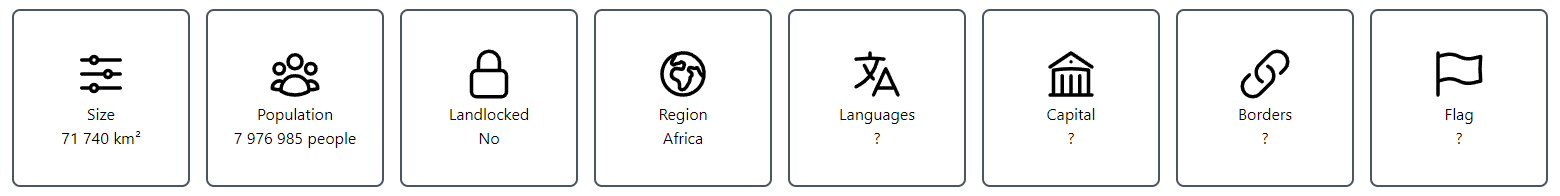
\includegraphics[width=.97\textwidth]{images/HintBoxes.jpg}
	\caption[HintBoxesComponent]{HintBoxesComponent - vlastní zpracování}
	\label{fig:angularhintboxes}
\end{figure}

Pokračujeme implementací komponenty country-guess-input, která uživateli umožní zadat svůj tip. 
Začneme šablonou, kde vytvoříme formulářový prvek pro zadání názvu země a~potvrzovací tlačítko. 
Dále podmenu textového pole, které zobrazí nejpodobnější země na základě zadaného textu -- filtrované země a~chybové hlášky. 
Můžeme také rovnou přidat obslužné metody pro akce a~události nad formulářem, které následně postupně doimplementujeme.

\begin{figure}[htb]
	\centering
		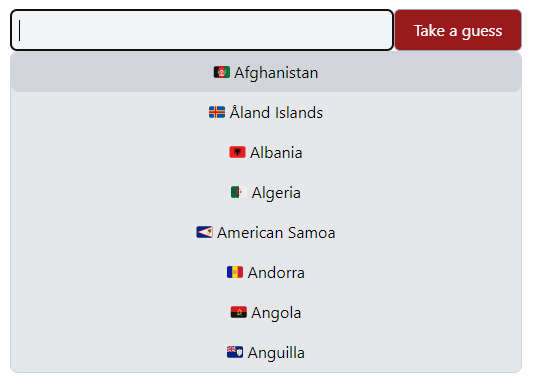
\includegraphics[width=.5\textwidth]{images/CountryGuessInput.jpg}
	\caption[CountryGuessInputComponent]{CountryGuessInputComponent - vlastní zpracování}
	\label{fig:angularcountryguessinput}
\end{figure}

V~souboru \emph{country-guess-input.component.ts}, tedy v~rámci třídy CountryGuessInputComponent, při změně vstupních vlastností (v~hooku \emph{OnChanges}) aktualizujeme vlastnost \emph{countriesWithoutAlreadyGuessed} a~\emph{filteredCountries}. 
V~případě první vlastnosti jde o~pole všech zemí bez těch, které uživatel již hádal. Druhá vlastnost poté představuje pole počátečních 8 prvků vlastnosti \emph{countriesWithoutAlreadyGuessed}. 
Metoda \emph{handleGuessButtonClick} zavolá obslužnou metodu rodičovské komponenty, která vyhodnotí tip a~aktualizuje stav hry. 
Aktualizujeme také hodnoty aktuálního tipu, filtrovaných zemí a~uzavřeme podmenu, k~čemuž slouží metoda \emph{handleChangeSelectedGuess} volaná i~napřímo z~šablony. 
Tělo metody \emph{handleInputChange} převede uživatelům tip do správného formátu a~pomocí převedené hodnoty aktualizuje aktuální tip spolu s~filtrovanými zeměmi.
Metoda \emph{handleKeyDown} se postará o~interakce s~podmenu pomocí klávesnice. Skrze šipky nahoru a~dolů povolíme uživateli vybrat hádanou zemi. 
Enter umožní změnu aktuálního tipu názvu země na právě tu, kterou uživatel označil v~podmenu. Escape poslouží k~uzavření podmenu.

Uvnitř pomocné metody \emph{updateGuessAndFilteredCountries} následně modifikujeme vlastnost \emph{currentGuess}. 
Dle metody \emph{getFilteredCountries} získáme aktuálně filtrované země na základě uživatelova tipu. 
Rovněž přenastavíme vlastnost \emph{isValidGuess}, která určuje, zda je uživatelův tip validní (taková země existuje). 
V~neposlední řadě aktualizujeme vlastnost \emph{selectedGuessIndex}, jež určuje, která země je vybraná v~podmenu. 
K~tomu slouží metoda \emph{clampSelectedGuessIndex}, která index udrží v~požadovaném rozmezí (0 až počet filtrovaných zemí).
V~metodě \emph{getFilteredCountries} získáme filtrované země na základě vlastnosti \emph{currentGuess}. 
Metoda \emph{changeSelectedGuessIndex} aktualizuje vlastnost \emph{selectedGuessIndex} o~hodnotu předanou v~argumentu. 
K~převodu tipu uživatele slouží pomocná metoda \emph{convertToFormattedGuess}. Metoda zajistí, aby tip začínal velkým písmenem a~zbytek řetezce byl složen z~malých písmen.

Implementujeme komponentu guessed-countries-list, jenž zobrazí seznam již hádaných zemí. 
Mezi vstupními vlastnostmi bude pole všech zemí (\emph{countries}), pole hádaných zemí uživatelem (\emph{guessedCountries}) a~také země, kterou uživatel musí uhodnout (\emph{randomCountry}).
Pomocí vstupních vlastností a~služby EnrichGuessedCountriesService získáme pole hádaných zemí s~jejich vlajkou a~vzdáleností od \emph{randomCountry} (\emph{distanceFromRandomCountry}).
Služba EnrichGuessedCountriesService ke každé hádané zemi přidá její vlajku a~vypočte hodnotu \emph{distanceFromRandomCountry}. 
Pro vypočtení vzdálenosti použijeme funkci \emph{getDistanceBetweenTwoPoints} a~vlastnost \emph{latlng}, kterou získáme ze serveru při získávání všech zemí. 
Funkci \emph{getDistanceBetweenTwoPoints} importujeme z~knihovny \emph{calculate-distance-between-coordinates} \cite{distancebetweencoordinates}. 
Hodnotu vlastnosti \emph{enrichedGuessedCountries} aktualizujeme v~rámci hooku \emph{OnChanges}. Seznam hádaných zemí vykreslíme v~šabloně.

\begin{figure}[htb]
	\centering
		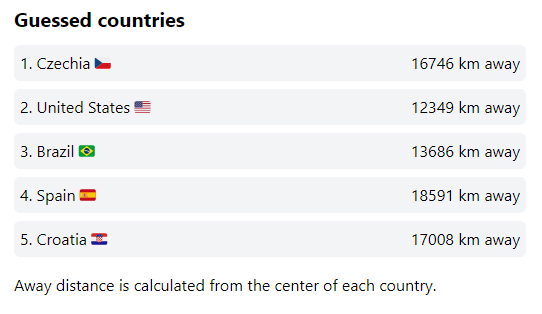
\includegraphics[width=.7\textwidth]{images/GuessedCountriesList.jpg}
	\caption[GuessedCountriesListComponent]{GuessedCountriesListComponent - vlastní zpracování}
	\label{fig:angularguessedcountrieslist}
\end{figure}

Pokračujeme implementací modálních oken, které se zobrazí při výhře či prohře. 
Vlastnosti \emph{isWinModalOpen} a~\emph{isLoseModalOpen}, určující, zda se mají okna zobrazit, bychom měli aktualizovat v~metodě \emph{handleEvaluateGuessAndUpdateState} v~CountryGuesserComponent. 
Oběma modálním oknům předáme vlastnost \emph{randomCountry} a~output \emph{handleClose} v~podobě obslužné události, která se vyvolá při zavření modálního okna. 
Do výherního modálu rovněž poskytneme vstupní vlastnost \emph{totalGuessesNeeded}, jíž využijeme v~obsahu okna. 
Obě modální okna budou velice podobné, a~proto vytvoříme komponentu base-modal, která bude sloužit jako šablona pro obě okna. 
BaseModalComponent bude přijímat titulek, obsah modálního okna a~\emph{handleClose} jako výstupní vlastnost. 
Šablona base-modal pak vykreslí základní strukturu modálního okna, s~dynamicky nastaveným titulkem, obsahem a~obslužnou metodou volanou při zavření modálního okna.

\begin{flushleft}
  \textbf{Routování a layout aplikace}
\end{flushleft}

Demonstrační aplikace bude složena z~hlavičky, patičky a~samotného obsahu, v~němž se vykreslí jednotlivé komponenty. 
Mezi jednotlivými stránkami se uživatel bude moci přepínat pomocí navigačního menu.

K~routování mezi jednotlivými stránkami využijeme modul Router přímo od Angularu. Nejprve vytvoříme cesty (\emph{routes}) pro jednotlivé stránky v~souboru \emph{app.routes.ts}. 
Proměnnou \emph{routes} vytvoříme dle předpisu \emph{Routes} a~následně exportujeme. Cesty pak poskytneme routeru v~rámci \emph{app.config.ts}.

\begin{prog}
// Část souboru app.routes.ts

import \{Routes\} from '@angular/router';

export const routes: Routes = [
  \{
    title: 'Home',
    path: '',
    component: LandingComponent,
    pathMatch: 'full',
  \},
  \{
    title: 'Counter',
    path: 'counter',
    component: CounterComponent,
  \},
  // Další cesty...
  \{path: '**', component: PageNotFoundComponent\},
];

// Část souboru app.config.ts

export const appConfig: ApplicationConfig = \{
  // V tomto nastavení poskytujeme služby a poskytovatele pro celou aplikaci.
  providers: [
    provideRouter(routes),
    // Další poskytované služby...
  ],
\};
\end{prog}

Pokračujeme vytvořením požadované struktury stránek v~AppComponent. Šablona bude obsahovat hlavičku, patičku a~obsah, který vykreslíme pomocí elementu \emph{router-outlet}. 

\begin{prog}
// Soubor app.component.html

<div class="min-h-screen flex flex-col">
  <app-header />

  <main class="flex-grow p-8">
    <!-- Router-outlet vykresluje šablonu (komponentu) pro aktuální URL adresu. -->
    <router-outlet></router-outlet>
  </main>

  <app-footer />
</div>
\end{prog}

V~rámci komponenty hlavičky pak vytvoříme navigační menu, které bude obsahovat odkazy na jednotlivé stránky. 
Můžeme se inspirovat například architekturou a~vzhledem navigačního menu Flowbite\footnote{Flowbite poskytuje pestrou sadu UI komponent založených na TailwindCSS.\cite{flowbitetwheader}}. 
Pokračujeme vypsáním všech cest aplikace, k~čemuž využijeme direktivy \emph{routerLink}, \emph{routerLinkActive}, \emph{routerLinkActiveOptions} a~referenci \emph{\#link}. 
Do \emph{routerLink} předáme patřičnou cestu a~\emph{routerLinkActive} umožní naslouchat na aktuální URL. Direktiva \emph{routerLinkActiveOptions} pak přepíše výchozí nastavení \emph{routerLinkActive}.
Díky referenci \emph{\#link} získáme informaci o~tom, zda je odkaz aktivní. To využijeme při podmíněném nastavení správných CSS tříd na aktivních a~neaktivních odkazech.

\begin{prog}
// Část souboru header.component.html

@for (route of appRoutes; track route.title) \{
  <li>
    <a
      [routerLink]="route.path"
      routerLinkActive
      [routerLinkActiveOptions]="routerLinkActiveOptions"
      #link="routerLinkActive"
      class="block py-2 pr-4 pl-3 lg:p-0"
      [ngClass]="\{
        'STATICKÉ STYLY PRO AKTIVNÍ ODKAZ...': link.isActive,
        'STATICKÉ STYLY PRO NEAKTIVNÍ ODKAZ...': !link.isActive
      \}"
      ariaCurrentWhenActive="page"
    >
      \{\{ route.title \}\}
    </a>
  </li>
\}
\end{prog}

Přepínání barevného režimu, otevírání a~zavírání mobilní navigace implementujeme pomocí obslužných metod a~vlastností třídy. 
Informaci o~tom, zda má uživatel zapnutý tmavý režim ukládáme do LocalStorage v~prohlížeči. 
Při kliknutí na tlačítko pro přepnutí režimu zavoláme metodu \emph{toggleDarkMode}, která změní hodnotu vlastnosti a~uloží ji do LocalStorage.

\begin{prog}
// Část souboru header.component.ts

protected toggleDarkMode(): void \{
  this.isDarkMode = !this.isDarkMode;
  this.updateDarkMode();
\}

private updateDarkMode(): void \{
  if (this.isDarkMode) \{
    document.documentElement.setAttribute('data-mode', 'dark');
    localStorage.setItem('data-mode', 'dark');
  \} else \{
    document.documentElement.removeAttribute('data-mode');
    localStorage.removeItem('data-mode');
  \}
\}
\end{prog}